documentclass{beamer}
\usepackage{fancybox}
\usepackage{beamerthemesplit}
\usepackage{hyperref}
\usepackage{comment}

\mode<presentation> {

\usetheme{Warsaw}
\setbeamertemplate{footline}[frame number]

  }
\title[Updated stock-recruitment DB]{The RAM II stock-recruitment database}
\subtitle{An historical and technological overview}
\author[Baum, Minto and Ricard]{Julia Baum \thanks{Scripps Institution of Oceanography, UCSD} \and Olaf Jensen \thanks{University of Washington} \and Coil\'{i}n Minto \thanks{Dalhousie University, Halifax NS, Canada} \and Daniel Ricard$^{3}$}

\date{Dec. 10th 2008 - NCEAS}

\begin{document}


\frame{\titlepage}
% [plain]


%\frame{\tableofcontents}

\section{Past}

\begin{frame}
\frametitle{RAM's original database}

\begin{itemize}
 \item A lifelong endeavour that started when RAM worked at DFO
 \item First summarised in a technical report and resulted in numerous publications
 \item Focused on:
\begin{itemize}
 \item Meta-analytic methods to draw strength from many stocks
 \item The relationship between spawning stock and recruitment 
 \item Maximum reproductive rate at low spawning stocks
\end{itemize}
 \item Housed in flat text files
\end{itemize}

Archived on server (i.e not updated anymore) and available from the following URL:\\
\url{http://chase.mathstat.dal.ca/~myers/welcome.html}

\end{frame}


\section{Present}
\begin{frame}
\frametitle{RAM II database - srdb}
\begin{itemize}
 \item A user-built database
 \item A relational database using the Open Source postgreSQL RDBMS with postGIS
 \item Internet accessible (TCP/IP), concurrent users, privileges and credentials
 \item Data from individual assessments are captured in a standardised spreadsheet file
 \item Suite of Open Source tools used for development (BASH, Perl, LaTeX, R, Python)

% \item Still under active development with more assessments being added and probably some design changes
\end{itemize}

\end{frame}


\begin{frame}[plain]
\frametitle{Database structure - Entity relationship diagram}
%\hspace*{-.6cm} \includegraphics[scale=0.18]{/Users/mintoc/docs/analyses/nceas/projects/doc/srdb-ERD.png}
\hspace*{-.6cm} \includegraphics[scale=0.18]{/home/srdbadmin/SQLpg/srDB/doc/srdb-ERD.png}
\end{frame}

%\begin{frame}
%\frametitle{Summary of database content, as of Dec. 10$^{\textnormal{th}}$ 2008}
% tot. num assessments by recorder, taxonomic order
% Geographic coverage (map)
% keep simple
%Changes daily whilst under active development
%\end{frame}

\begin{frame}[plain]
\frametitle{Geographic coverage}
\begin{center}
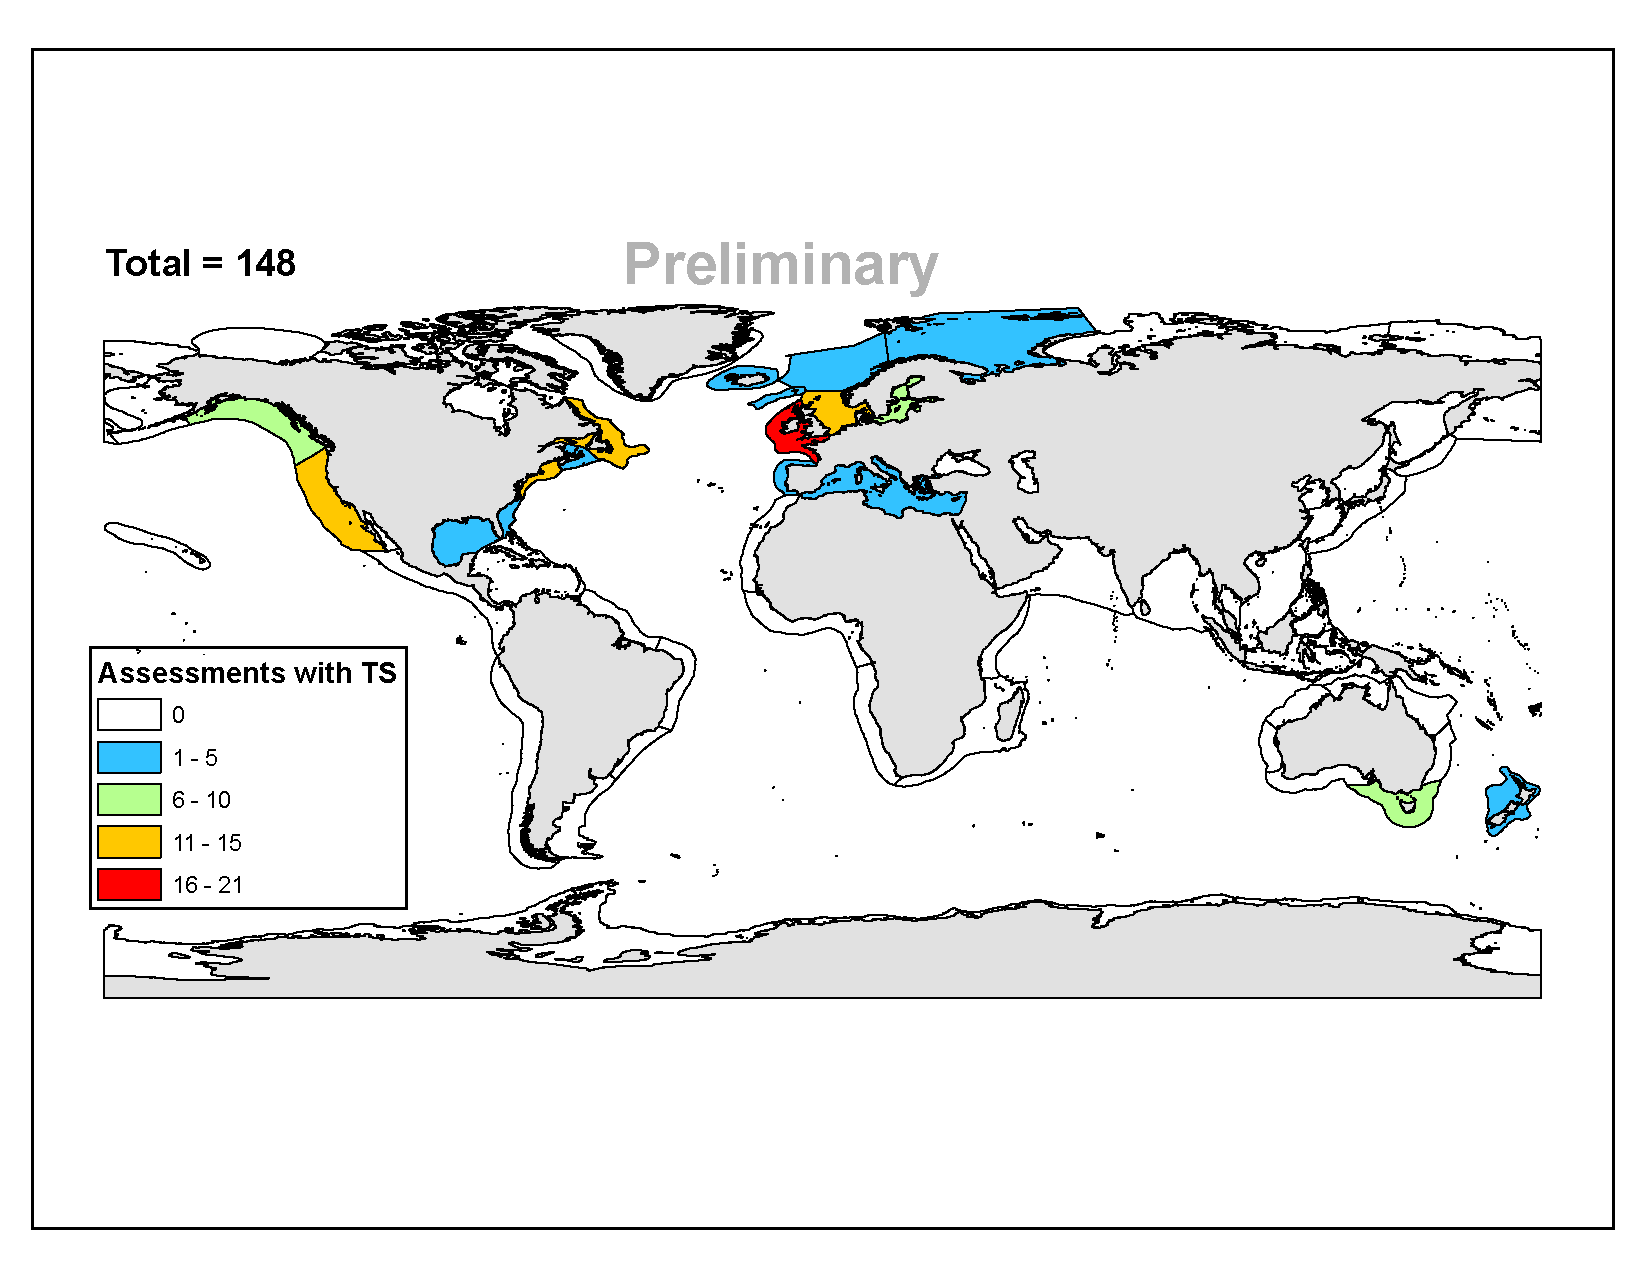
\includegraphics[width=10cm]{/home/srdbadmin/SQLpg/srDB/doc/Data_summary_by_LME.pdf}
\end{center}
\end{frame}

\begin{frame}[plain]
\frametitle{Entered assessments}
\begin{center}
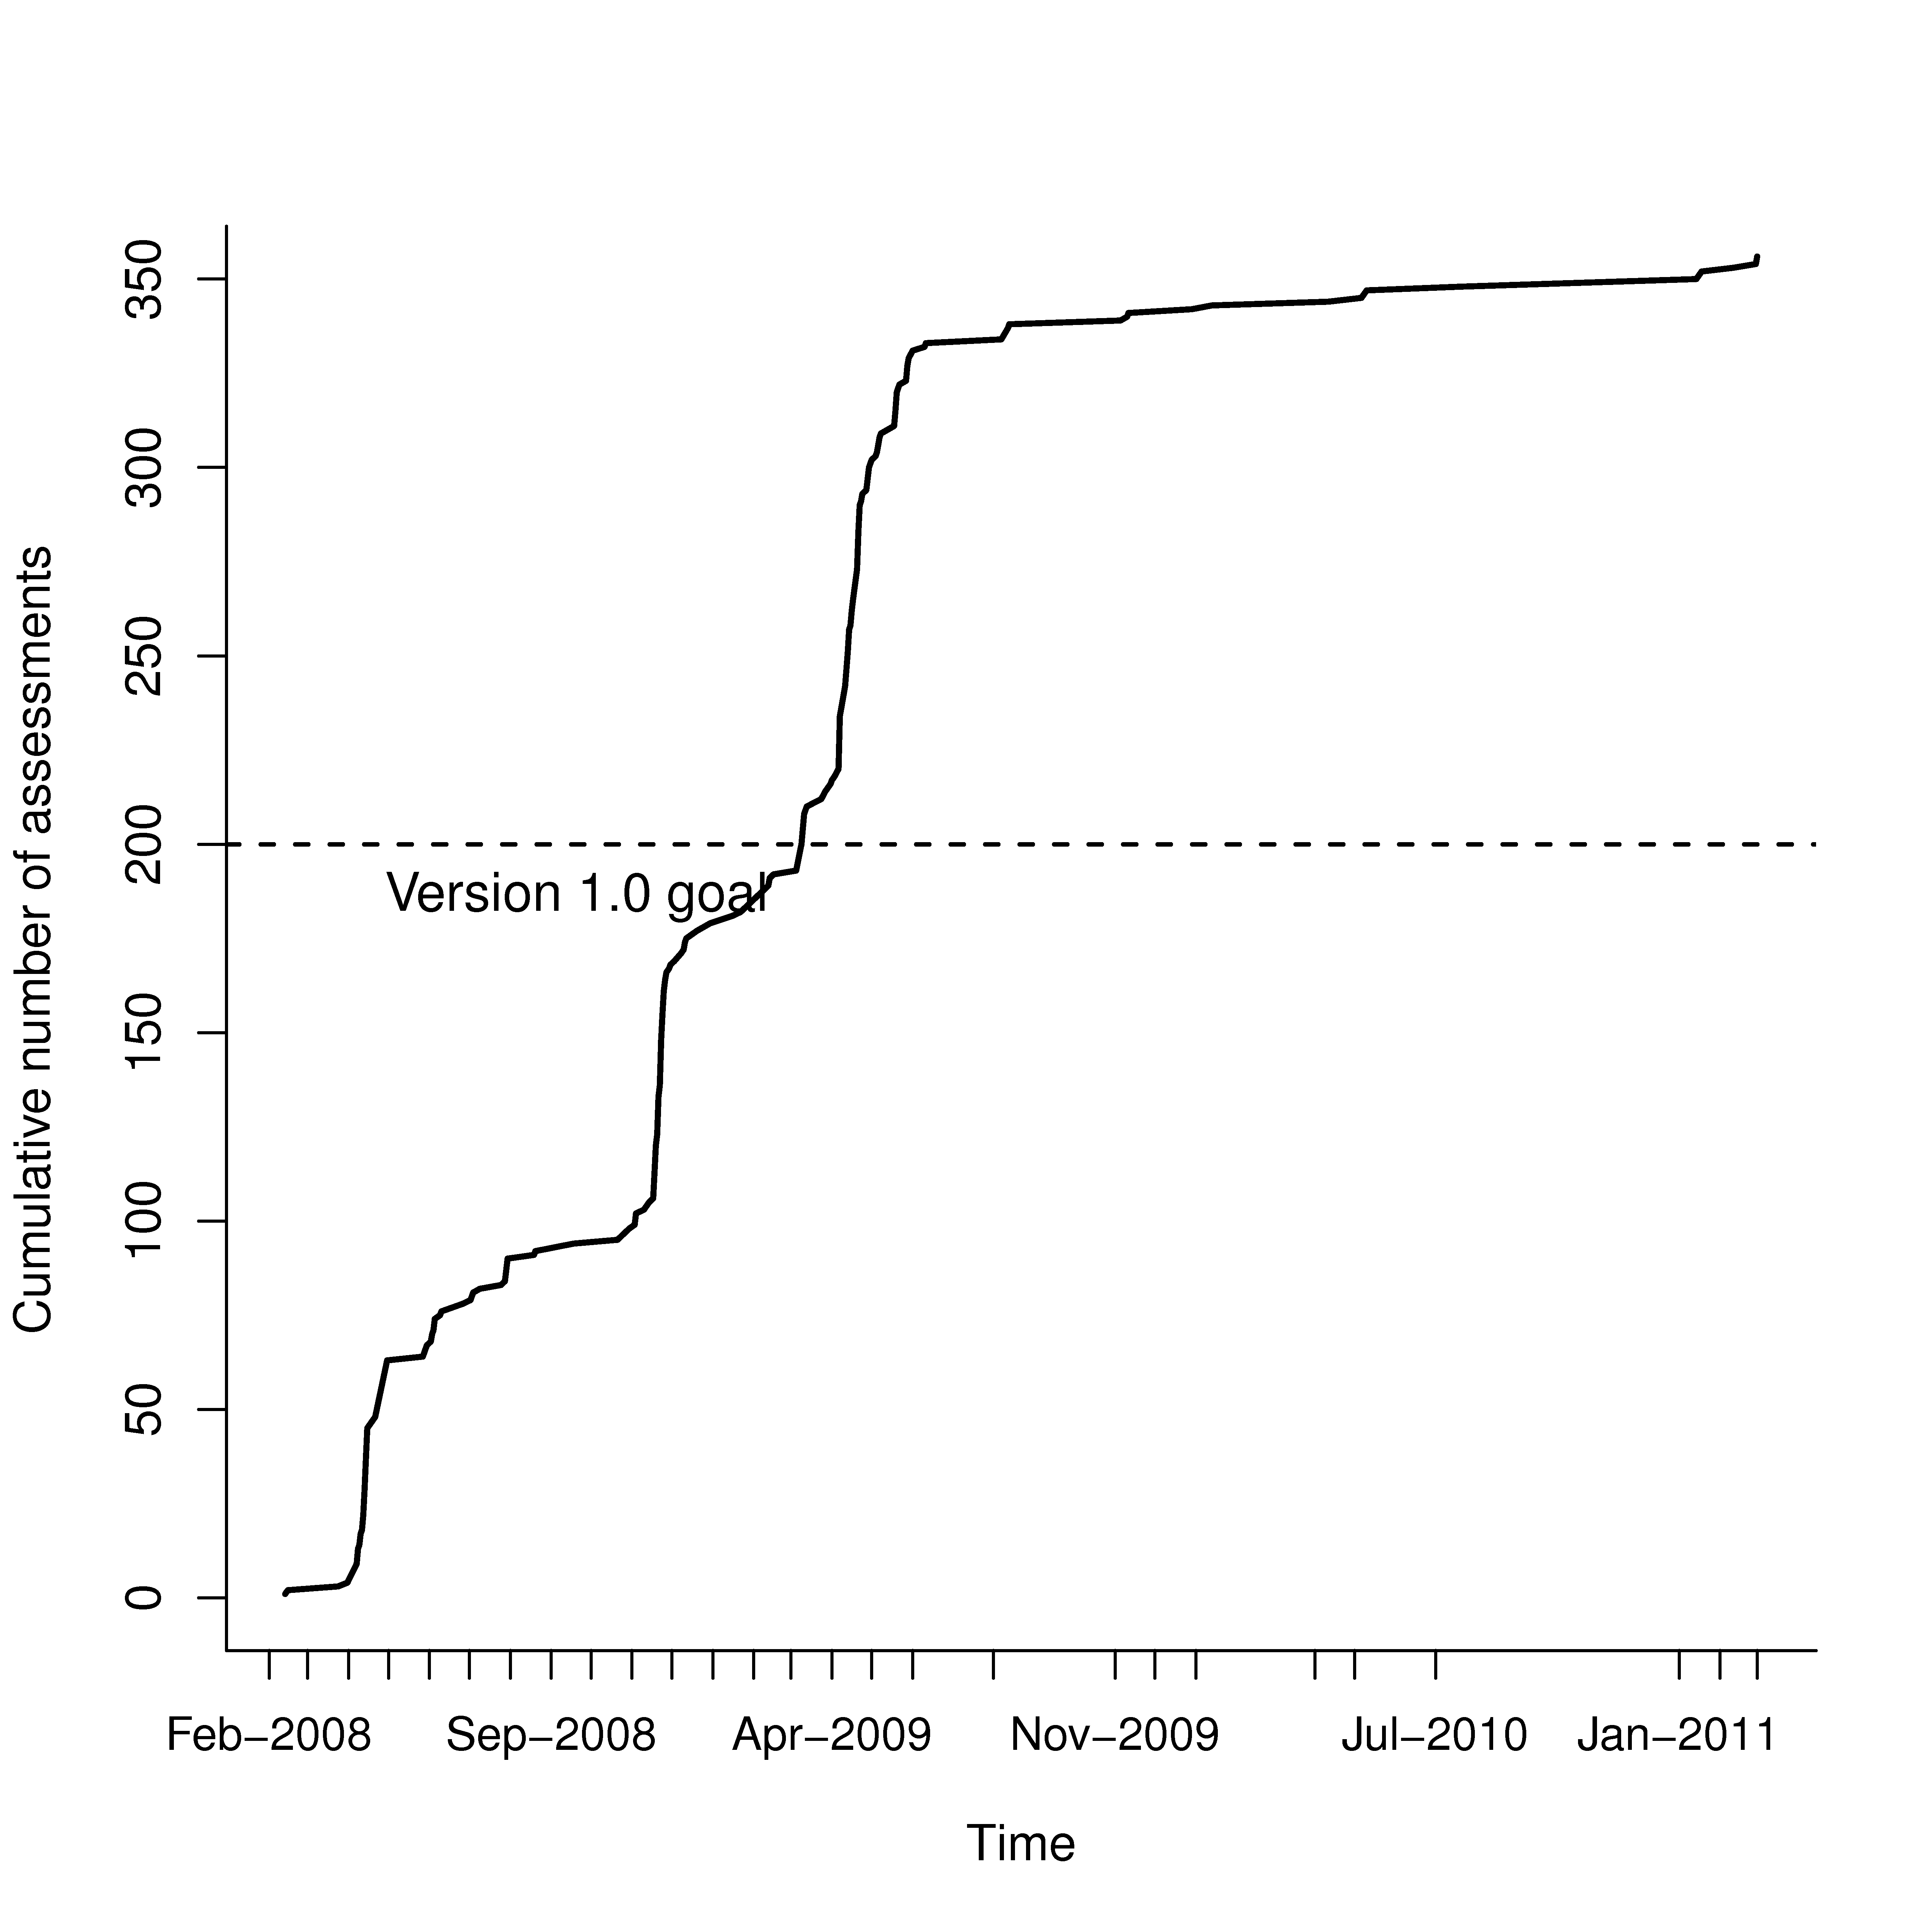
\includegraphics[width=8cm]{/home/srdbadmin/SQLpg/srDB/doc/timeseries_assess.png}
\end{center}
\end{frame}

\begin{frame}
\frametitle{Demo session}
RAMlegacy portal: \url{http://www.marinebiodiversity.ca/RAMlegacy}\\
\vspace{.5cm}
How to:
\begin{enumerate}
\item Submit an assessment
\item Track assessment progress
\item Connect to the database on
\begin{itemize}
\item[-] development server
%\item[-] local machine
\end{itemize}
\item Get the timeseries data
\item QCQA plot
%\item Plot the timeseries data %QC/QA script (run perl script)
\end{enumerate}
\end{frame}
\begin{comment}
\begin{frame}
\frametitle{Avoiding the pre-release snapshot}
\begin{description}
\item[Snaphot:]{A once-off, static copy of the database content}
\end{description}
Assessments continually being entered\\
Data errors are likely (snapshot still has errors)\\
Lacks reproducibility (database moves on)\\
\vspace{.5cm}
\begin{description}
\item[Live data:]{Feed directly from database to analytical software}
\end{description}
Analysis can be re-run from current version of the database \\
All researchers working from same page\\
Uses all available assessments\\
Data corrections ran at source
\end{frame}
\end{comment}

\section{Future}

\begin{frame}
\frametitle{Release of srdb version 1.0}
Points to consider before wide distribution and usage:
\begin{itemize}
 \item How to make this data authoritative? {\bf QC/QA}
 \item How to make this data citable? {\bf Metadata and summary publication}
 \item How to make analyses reproducible? {\bf Versioning of database content}
 \item How to ensure usability? {\bf Documentation, tailored database views as products}
 %\item Data access decisions? 
\end{itemize}
\vspace{.25cm}
Complete entry of top-twenty tonnage fisheries\\
\vspace{.25cm}
Anticipated formal release: {\bf March 2009}\\
\end{frame}
%\begin{frame}
%\frametitle{Source code and resources on subversion}
%\end{frame}
\begin{frame}
\frametitle{Longterm plans}
\begin{itemize}
\item Addition of stocks from other areas (Africa, South America, Asia), 
\item Addition of new species (salmonids, freshwater fishes, invertebrates)
\item Addition of ancillary data (management, economic, life history data.....)
\item Engage with regional fisheries agencies for timely inclusion of new assessments 
\item Develop a web-based interface for querying the database
\end{itemize}
\end{frame}

\begin{frame}
\frametitle{Acknowledgments}
Sincere thanks to:\\
\vspace{.5cm}
RAM \\
All assessment scientists\\ 
All recorders\\
NCEAS working group
\end{frame}
\end{document}
